\section{Introduction}
This document contains the requirements for the Android game \textit{Sea Battle}, an online two-player version of the famous \textit{Battleship} game, where one player targets coordinates on the enemy's map, and bombs that coordinate. The enemy's map is initially hidden from the player, but as it is bombed, it will be revealed. A ship has been sunk when all its cells have been hit. The game is over when all the enemy's ships are sunk. You can see the cover of the traditional board game in figure \ref{fig:battleship-boardgame}.
\newline
\newline
A \textit{game map} is a 10 x 10 grid. It contains the ships described in table \ref{tab:ships}, with given dimensions:

\begin{table} [h]
    \centering
    \begin{tabular}{l | c}
        Ship name & Dimension \\
        \hline
        Aircraft carrier & 5x1 \\
        Battleship & 4x1 \\
        Submarine & 3x1 \\
        Destroyer & 3x1 \\
        Patrol boat & 2x1 \\
    \end{tabular}
    \label{tab:ships}
    \caption{The ships and their size in the game of Battleship}
\end{table}

\begin{figure}[h]
  \centering
    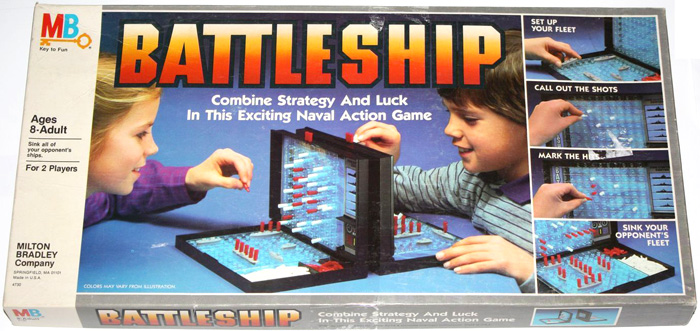
\includegraphics[width=300pt]{figs/battleship.jpg}
  \caption{The cover of the traditional boardgame Battleship}
  \label{fig:battleship-boardgame}
\end{figure}

Note that ships can be oriented either vertically or horizontally, but not diagonally.
\newline
\newline
We chose Battleship, because it is simple, and should not be too hard to implement. This will give us more time to focus on the architecture and network part of the game. We plan to make a \textit{matchmaking} system that will allow a user to either create a \textit{game room} and wait for another player to join, or join an existing game room. When there are two players in the same game room, the game will start.
\newline
\newline
We will begin the document by describing the functional requirements of our game, before we move on to the quality requirements, which will be described in scenarios. After that there will be a section on our COTS of choice, before we list references, issues and changes.